\documentclass[tikz,border=50mm]{standalone}
% !TeX program = luatex

%===This is the preambule I call in every file===

\usepackage{tikz}
\usepackage{xcolor}
\usepackage{pgfplots}
\usepackage{circuitikz}
\usepackage{tikz-3dplot}
\pgfplotsset{compat=newest}
\usetikzlibrary{arrows.meta, shapes.geometric, positioning, perspective, patterns.meta, decorations.pathreplacing, decorations.pathmorphing, decorations.markings, patterns, arrows.meta, shapes, shapes.geometric, decorations.text, angles, quotes,calc, 3d, math, circuits.ee.IEC,hobby, knots, intersections, through}


%=== The Euler Med Logo ===
%=== i.e. My signature ===

\usepackage{amsmath, amsfonts}
\makeatletter
\newcommand*\eulermed{{
\scalebox{3.3}{$\mathbb{E}$}\kern-1pt \scalebox{1.5}{u$\ell\varepsilon\rho$}\kern-55pt
\raisebox{19pt}{\scalebox{1.5}{$\mathcal{M}\varepsilon\delta$}}}
\@}
\makeatother

\begin{document}
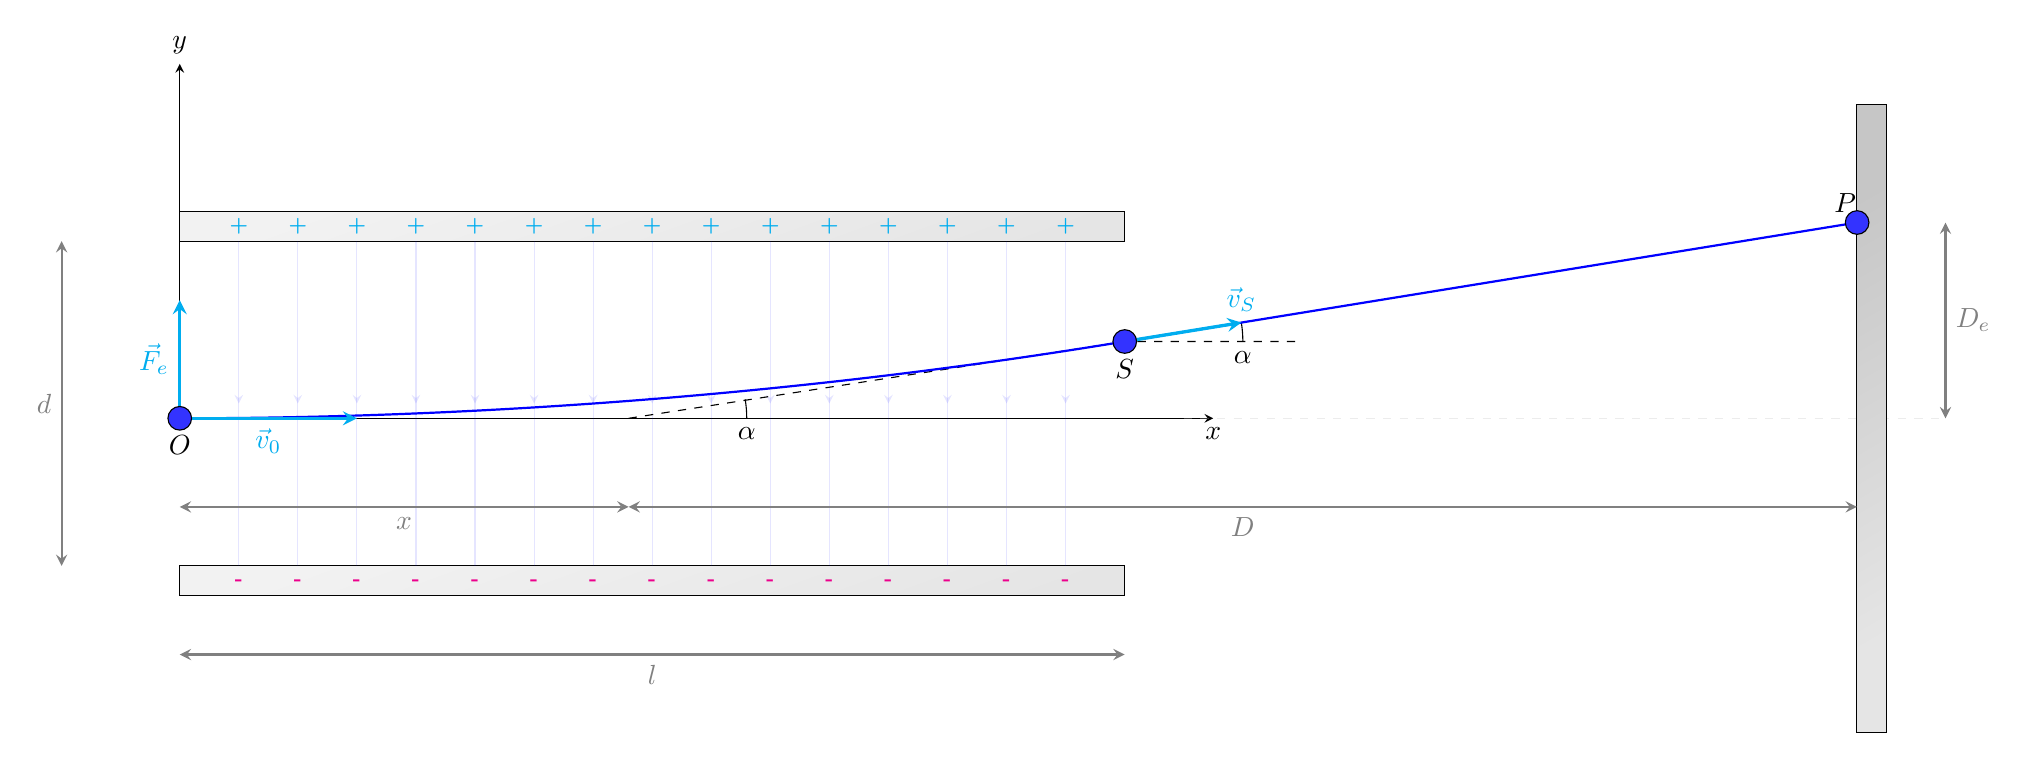
\begin{tikzpicture}[>=stealth,decoration={markings,mark=at position 0.5 with {\arrow{>}}}, scale=1.5]
%Constants~~~~~~~
\def\l{8} 
\def\d{3}
\def\x{3.8}
\def\D{10}
\def\sy{0.65}
\pgfmathsetmacro\px{\l-\x+\D}          
\pgfmathsetmacro\py{\sy+2*\sy*(\D-\x)/\l} 
\pgfmathsetmacro\a {atan(2*\sy/\l)}      
%Coordinates~~~~~~~
\coordinate (o)  at (0,0);
\coordinate (o') at (\px,0);
\coordinate (x)  at (\x,0);
\coordinate (s)  at (\l,\sy);
\coordinate (p)  at (\px,\py);
%the capacitor plates 
\foreach \i in {1.5, -1.5}{
\draw[top color=lightgray!20,bottom color=lightgray!40,shading angle=20] (0,\i)rectangle(\l,\i+0.25);
}
%their charges
\foreach \i in {.5,1,1.5,...,7.5}{
\node[scale=0.75, cyan] at (\i,1.625) {\bfseries +};
\node[scale=0.75, magenta] at (\i, -1.375) {\bfseries -};
}
%the axis 
\draw[->] (o)--(0,3) node[above] {$y$};
\draw[->] (o)--(\l+0.75,0) node[below] {$x$};
\draw[dashed, lightgray, opacity=0.3] (\l+0.5,0)--(\px+0.75,0);
%Electric field lines 
\foreach \i in {.5,1,1.5,...,7.5}{
\draw[postaction={decorate}, blue, opacity=0.1] (\i,1.5)--(\i,-1.25);
} 
\filldraw[top color=lightgray!90, bottom color=gray!20, shading angle=30] (\px,-\py-1)rectangle(\px+.25,\py+1);
%The other components 
\draw[dashed] (x)--(s)--++(1.5,0);
\foreach\i in {x,s}{
\draw ($(\i)+(\a:1)$) arc (\a:0:1) node [below] {$\alpha$};}
\draw[thick,gray, <->] (0,-2)--(\l,-2) node[below, midway] {$l$};
\draw[thick,gray, <->] (-1,-1.25)--(-1,1.5) node[midway, left] {$d$}; 
\draw[thick,gray, <->] (0,-0.75)--(\x,-0.75)node[below, midway] {$x$};
\draw[thick,gray,<->] (\x,-0.75)--(\px,-0.75)node[below, midway] {$D$};
\draw[thick,gray, <->] (\px+0.75,0)--(\px+0.75,\py) node[midway, right] {$D_e$};
%the trajectory 
\draw[blue, thick] (o) parabola (s)--(p);
%The electric force and velocity 
\draw[very thick, cyan, ->] (o)--(1.5,0) node[below, midway] {$\vec{v}_0$};
\draw[very thick,cyan,->] (s) -- ($(s)!1cm!(p)$) node[above] {$\vec{v}_S$};
\draw[very thick, cyan, ->] (o)--(0,1) node[left, midway] {$\vec{F}_e$};
%the charge positions 
\foreach \i/\j in {o/$O$, s/$S$}{
\draw[fill=blue!80!white] (\i)circle(0.1) node[below=0.1] {\j};
}
\draw[fill=blue!80!white] (p)circle(0.1) node[left=0.15, above] {$P$};
\end{tikzpicture}
\end{document}
